\documentclass{article}
\usepackage[T1]{fontenc}
\usepackage{lmodern}
\usepackage{graphicx}
\usepackage{amsmath,amssymb}
\usepackage[a4paper,margin=2cm]{geometry}
\usepackage[absolute,overlay]{textpos}
\setlength{\TPHorizModule}{1mm}
\setlength{\TPVertModule}{1mm}
\usepackage[indonesian]{babel}
\usepackage{hyperref}
\setlength{\emergencystretch}{2em}
% unit: Halaman 22

\begin{document}

% === Halaman 22 (python/native) ===

• Demo Merkle-Hellman knapsack online: 

https://asecuritysite.com/encryption/knapcode?val1=3\%2C\%205\%2C\%2015\%2C

\%2025\%2C\%2054\%2C\%20110\%2C\%20225\&val2=10\&val3=439\&val4=100100011

0010111011001101111 

22

% deskripsi: gambar native xref 97
\noindent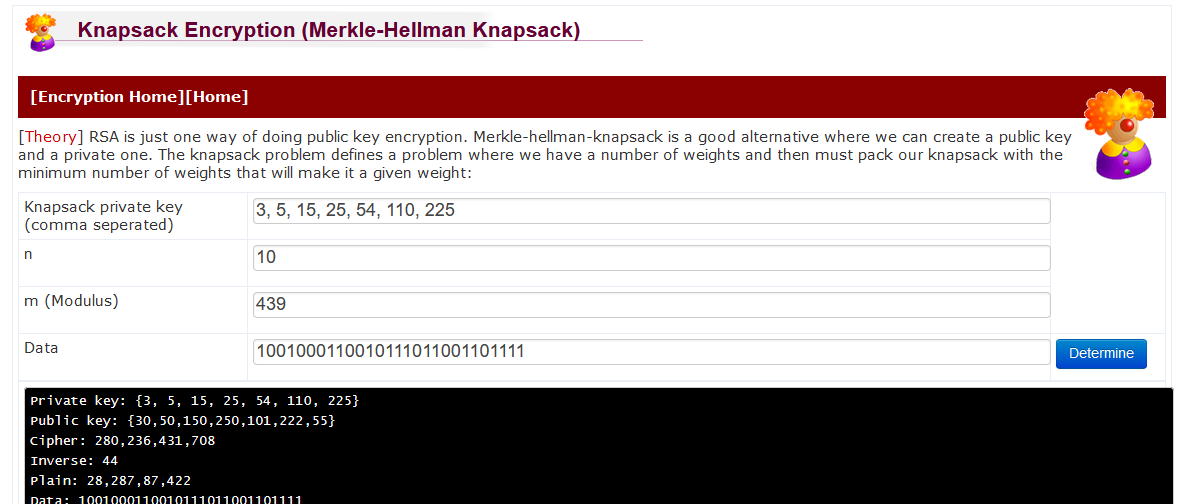
\includegraphics[width=0.85\textwidth]{../../images/python/page_022_img_01.png}

\end{document}
